\documentclass[conference]{IEEEtran}
\IEEEoverridecommandlockouts
% The preceding line is only needed to identify funding in the first footnote. If that is unneeded, please comment it out.
\usepackage{cite}
\usepackage{amsmath,amssymb,amsfonts}
\usepackage{graphicx}
\usepackage{textcomp}
\usepackage{hyperref}
\usepackage{url}
\usepackage{xcolor}
\usepackage{subcaption}
\def\BibTeX{{\rm B\kern-.05em{\sc i\kern-.025em b}\kern-.08em
    T\kern-.1667em\lower.7ex\hbox{E}\kern-.125emX}}
\begin{document}

\title{\emph{NautDB}: Towards a Hybrid Runtime for Processing Compiled Queries
\thanks{This work was supported by NSF Award \#1640864. Opinions, findings and conclusions expressed in this material are those of the authors and do not necessarily reflect the views of the National Science Foundation.}
}

\author{\IEEEauthorblockN{Samuel Grayson}
\IEEEauthorblockA{\textit{Department of Computer Science} \\
\textit{University of Texas at Dallas}\\
samuel.grayson@utdallas.edu}
% \and
% \IEEEauthorblockN{Kyle Hale}
% \IEEEauthorblockA{\textit{Department of Computer Science} \\
% \textit{Illinois Institute of Technology}\\
% khale@cs.iit.edu}
% \and
% \IEEEauthorblockN{Boris Glavic}
% \IEEEauthorblockA{\textit{Department of Computer Science} \\
% \textit{Illinois Institute of Technology}\\
% bglavic@iit.edu}
}

\newcommand{\todo}[1]{\textcolor{red}{#1}}

\maketitle

\begin{abstract}
General purpose operating and database system suffer from their generality which makes achieving optimal performance extremely hard, especially on modern hardware.
The goal of this research is to integrate specialization techniques from the OS community (hybrid runtimes) and DB community (compiled queries) for high-performance query processing on modern hardware. We envision a system called \emph{NautDB}, a hybrid dataflow runtime for executing compiled queries. As a first step towards our goal we use a simple prototype to evaluate the performance of compiled queries on Linux and run as a \emph{Nautilus} hybrid runtime.
Our results demonstrate that combining these specialization techniques has transformative potential for building the next generation (distributed) high-performance query processing systems and big data platforms.
\end{abstract}

\begin{IEEEkeywords}
hybrid runtimes, light-weight kernels, compiled query processing, high-performance query processing
\end{IEEEkeywords}

%%%%%%%%%%%%%%%%%%%%%%%%%%%%%%%%%%%%%%%%
\section{Introduction}

  Both the operating system (OS) and database (DB) communities have strived to build general purpose systems which exhibit reasonable performance for a wide variety of applications and are user-friendly.
  %
  However, the performance of general purpose operating and database systems suffers from being overly generic and from hiding implementation details behind multiple layers of abstraction~\cite{GICEVA:2016:OS_SUPPORT}.
  %
Both communities have worked on achieving better performance on modern hardware without sacrificing ease of use. Specifically, OS researchers have introduced hybrid runtimes~\cite{HALE:2017:MULTIVERSE,HALE:2016:MULTIVERSE,HALE:2015:NAUTILUS,HALE:2016:HRTHVM} as a means to give an application more immediate access to hardware and control over OS behavior while database researchers have studied query compilation to specialize a database execution engine to a particular query~\cite{SK16,N11}.

The ultimate goal of this research is to integrate, for the first time, these specialization techniques from the OS community (hybrid runtimes) and DB community (compiled queries) for high-performance query processing.
  %
As a first step towards this goal, we build a testing prototype that uses hand-optimized query operator implementations and use this prototype to evaluate the potential performance benefit of running compiled queries as a hybrid runtime.
%
Our preliminary results demonstrate that, even though this first version of our prototype is still quite naive, we can achieve better and more predictable performance through specialization.
%


% %%%%%%%%%%%%%%%%%%%%%%%%%%%%%%%%%%%%%%%%
% \section{Related Work}



%%%%%%%%%%%%%%%%%%%%%%%%%%%%%%%%%%%%%%%%
\section{Preliminary Evaluation}

As a preliminary assessment of the potential of our idea, we have built an initial prototype consisting of manually optimized implementations of common database query operators.
We then evaluate the performance of this prototype on a standard Linux distribution and embedded into the Nautilus aerokernel~\cite{HALE:2015:NAUTILUS}.
The purpose of this experiment is to evaluate how specialized implementations of OS functionality (e.g., memory management) and the immediate control over hardware might benefit evaluation of compiled query plans (like the ones already produced by modern query compilers used in main memory database systems~\cite{N11}).

%%%%%%%%%%%%%%%%%%%%%%%%%%%%%%%%%%%%%%%%
\subsection{Testing Prototype}
\label{sec:testing-prototype}

Our prototype supports several important database operators including selection, projection, and sort. Our implementation stores data in columnar chunks: the table is split into chunks of rows, which are stored column-at-a-time. Here we focus on the implementation of the sort operator, because this operator is used to implement other operators like aggregation and joins (merge-join). Our sort implementation uses counting sort to sort the data within a chunk and merged sort to sort across chunks. We have implemented a row-oriented and a column-oriented variant of this sort algorithm.

%%%%%%%%%%%%%%%%%%%%%%%%%%%%%%%%%%%%%%%%
\subsection{Experimental Setup}
\label{sec:experimental-setup}

We ran our prototype on Linux (linux kernel 4.17.6) and as a hybrid runtime using Nautilus\footnote{\url{https://github.com/HExSA-Lab/nautilus} - git commit \texttt{2fb4e52816}}~\cite{HALE:2015:NAUTILUS,HALE:2016:HRTHVM}.
All experiments were run on a 16-core x86\_64 AMD EPYC machine with 4 NUMA nodes.
We sort a table consisting of $256$ chunks varying the number of elements\footnote{elements are stored as \texttt{uint32\_t} values} per chunk and the number of columns in the table.

%%%%%%%%%%%%%%%%%%%%%%%%%%%%%%%%%%%%%%%%
\subsection{Experimental Results}
\label{sec:experimental-results}



%%%%%%%%%%%%%%%%%%%%%%%%%%%%%%%%%%%%%%%%
\begin{figure*}[t]
  \centering
  \begin{minipage}{0.31\linewidth}
    \centering
    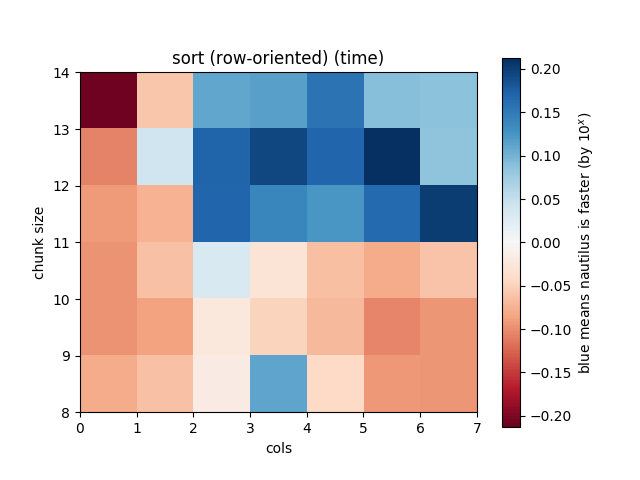
\includegraphics[width=1\linewidth]{../plots/sort_2d.png}
    \subcaption{Row-oriented sorting for a table with 256 chunks and up to  $128$ columns}\label{fig:sort2d}
  \end{minipage}
  \hspace{0.01\linewidth}
  \begin{minipage}{0.31\linewidth}
    \centering
  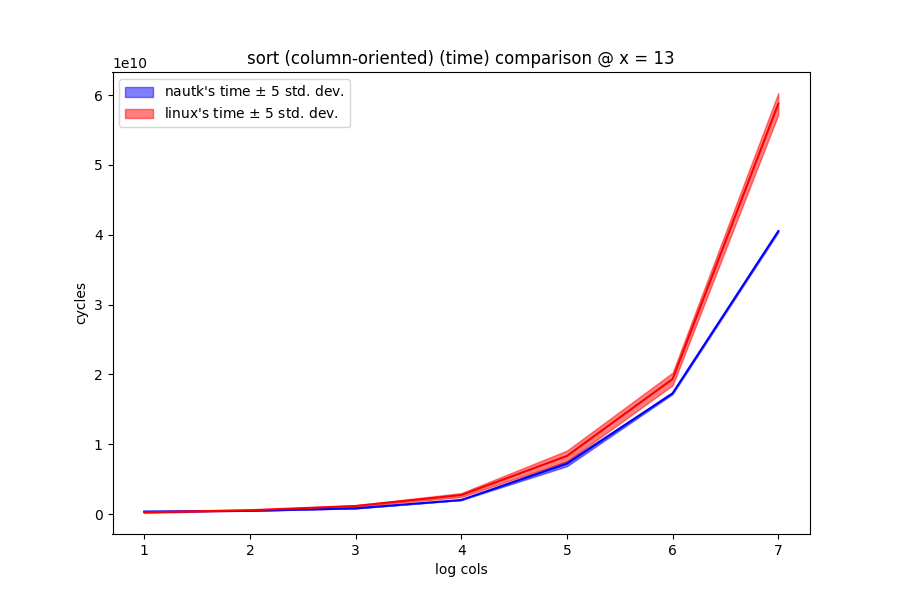
\includegraphics[width=1\linewidth]{../plots/sort.png}
    \subcaption{Column-oriented sort measuring runtime and uncertainty for a fixed chunk size ($2^{13} = 8192$), varying the number of columns}\label{fig:colsort}
  \end{minipage}
  \hspace{0.01\linewidth}
  \begin{minipage}{0.31\linewidth}
    \centering
      \begin{tabular}{l || r | p{1.6cm} }
        \textbf{Kernel}    & TLB misses  & Instruction cache misses \\[1mm]
        \hline\hline&&\\[-2mm]
        \textbf{Linux}     & 135,000,000 & 3,030,000 \\[2mm]
         \textbf{Nautilus} &           1 &   480,000 \\[2mm]
      \end{tabular}

    \subcaption{TLB and cache misses for row-oriented sorting of a $128$ column table with $8192$ elements per chunk}\label{fig:cache_miss}
  \end{minipage}

\caption{Evaluating the performance of sort on Nautilus and Linux.}
  \label{fig:perf-eval}
\end{figure*}
%%%%%%%%%%%%%%%%%%%%%%%%%%%%%%%%%%%%%%%%

The results of these experiments are shown in Figure~\ref{fig:perf-eval}. For larger number of columns and larger chunks, Nautilus (with relatively low developer-effort) outperforms Linux. This is because Nautilus has larger page size and incurs less TLB misses (see Table \ref{fig:cache_miss}). Furthermore, note (Figure~\ref{fig:colsort}) that performance in Nautilus is much more predictable than in Linux. This effect is observed even in configurations where Linux outperforms Nautilus. This is because Nautilus does not have scheduling interrupts, so it avoids unpredictable detours which also leads to better cache performance.


%%%%%%%%%%%%%%%%%%%%%%%%%%%%%%%%%%%%%%%%
\subsection{Discussion}
\label{sec:discussion}


These preliminary result demonstrate that specialization allows us to tune both the OS and DB engine to a query workload and that compiled queries that consist of highly-specialized code benefit from a hybrid runtime environment.
Furthermore, hybrid runtimes have much more predictable performance than general purpose OSes which will improve performance of bulk-synchronous parallel algorithms.
Our prototype based on the \emph{Nautilus} aerokernel does outperforms Linux in some parameter settings, despite our comparatively low developer-effort (Linux has been maturing for decades).
%This is even though the research prototype implementation of OS features in Nautilus has to compete with a mature industrial strength implementation in Linux that has been optimized by a large number of skilled developers over decades.

%%%%%%%%%%%%%%%%%%%%%%%%%%%%%%%%%%%%%%%%
\section{Our Vision for NautDB}
\label{sec:our-vision-nautdb}

As a long term goal, we envision to build \emph{NautDB}, a hybrid dataflow runtime which executes tasks that are represented as compiled (machine) code. The frontend of NautDB will be a query compiler that translates high-level queries (SQL or another  high-level and data-centric language) into compiled low-level tasks to be executed by the runtime. The present paper represents the first important step towards this goal.


%%%%%%%%%%%%%%%%%%%%%%%%%%%%%%%%%%%%%%%%
\section{Conclusions and Future Work}
\label{sec:concl-future-work}

This work demonstrated the potential of combining hybrid runtimes with compiled query processing. In future work, we plan to evaluate additional database operators, parallel execution of such operators, and evaluate how performance is affected by environmental noise from other applications running at the same time.

%%%%%%%%%%%%%%%%%%%%%%%%%%%%%%%%%%%%%%%%
  \bibliographystyle{abbrv}
  \bibliography{../kyle,../sam,../boris}


\end{document}

%%% Local Variables:
%%% mode: latex
%%% TeX-master: t
%%% End:
